{
\subsection{Eksperimentsopstilling}
I \ref{chap_afproevning} er de optimale tærskelværdier fundet.
Idet denne hypotese blot kigger på frekvensen for brug af det gyldnesnit
mod andre snit, hvis eneste restriktion er at de skal have et fælles
forhold til det gyldnesnit.
Det er også fordelagtigt at maksimere antallet af andre snit, da det
giver et bedre grundlag for eksperimentet.
Afstanden mellem to snit er begrænset af margin defineret til at være
$2.4\%$\ref{margin}. 
Denne margin skal være tilstede på begge sider af et snit, så derfor vil
hvert snit fylde $(2.4*2)\%$.
Det maksimale antal af snit på et billede må altså være
$100/4.8=20.833$. Hvilket ses på denne figur \ref{snitogmargin}
\begin{figure}[ht]
	\begin{center}
		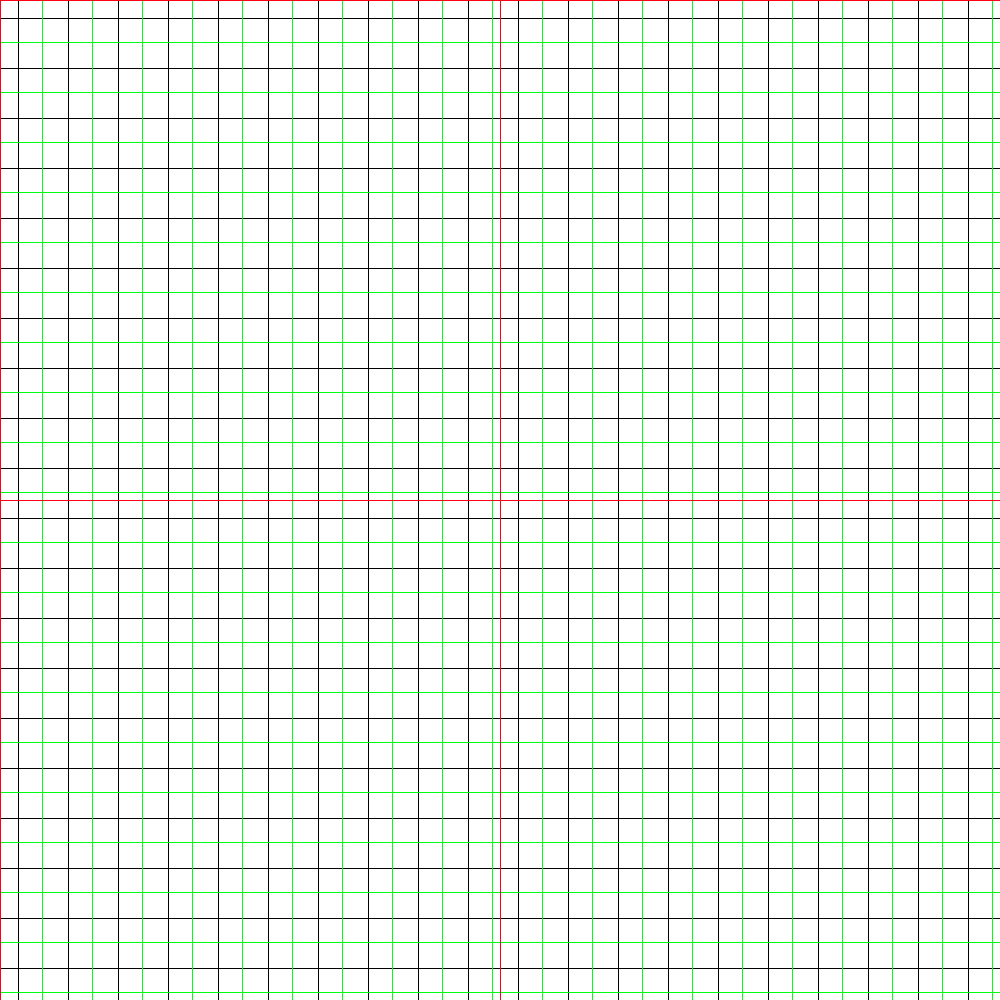
\includegraphics[scale=0.3]{afsnit/resultater/billeder/20_cuts_med_margin}
	\end{center}
	\caption{Sort:snittene, grøn: margins og rød er midten}
	\label{snitogmargin}
\end{figure}
Yderpunkterne $0.958$ og $0.518$ er problematiske, $0.958$'s margin
løber udover billedet, dvs. at den ren principielt går glip af at
detektere en masse interessante regioner.
$0.518$ lider af det modsatte problem, den kan potentielt fange
interessante regioner, på begge sider af midten.
For at være helt præcis så er det i $0.518$ tilfælde:\\
$1-0.518 = 0.482$
$0.518-0.482=0.036$\\
Hvilket er afstanden mellem de to snit.
Der er altså en stimmel på $0.05-0.036 = 0.014 = 1.4\%$ af billedet,
hvor interessante regioner bliver talt to gange.

\subsection{Resultater}
Vi har kørt vores analyse på $17,364$ billeder, men i vores resultater
sorterer vi $2,989$ af disse fra, da de kun er udsnit af et større maleri.
Som vist i tabel \ref{tabel_fjern_detaljer} herunder, er dette en nedgang
på $17.21$ procent og vi har $14,375$ brugbare resultater tilbage.

\begin{table}[H]
    \centering
    \begin{tabular}{r@{\ \ }p{12em}r|r@{.}l}
            & Analyserede malerier & $17,364$ & $100$ & $00\%$   \\
        $-$ & Udsnit af malerier   &  $2,989$ &  $17$ & $21\%$   \\\hline
            & Resultater           & $14,375$ &  $82$ & $79\%$
    \end{tabular}
    \caption[]{Udregning af brugbare resultater.}
    \label{tabel_fjern_detaljer}
\end{table}

Af de brugbare resultater, ser vi i tabel \ref{tabel_fordeling}, at der
i $91.43$ procent af malerierne er fundet mindst én region som ligger i
det gyldne snit. Vi kan derfor ikke afvise hypotese \ref{hypo_binaer}.

\begin{table}[H]
    \centering
    \begin{tabular}{r@{\ \ }p{12em}r|r@{.}l}
            & Positive resultater   & $13,143$ &  $91$ & $43\%$ \\
        $+$ & Negative resultater   &  $1,232$ &   $8$ & $57\%$ \\\hline
            & Resultater i alt      & $14,375$ & $100$ & $00\%$
    \end{tabular}
    \caption[]{Et positivt resultat beskriver et maleri, hvori der er
    fundet mindst én region, som ligger i det gyldne snit. Et negativt
    resultat er et maleri, hvori der ikke findes nogen regioner, som
    ligger i det gyldne snit.}
    \label{tabel_fordeling}
\end{table}

Vi undersøger nu, hvor mange af de brugbare resultater, som er forsynet
med dimensioner i databasen, således at vi kan undersøge, hvorvidt
lærredet er konstrueret som et gyldent rektangel. Udregningen i tabel
\ref{tabel_med_dimensioner} viser, at ud af de brugbare resultater,
mangler $2,410$ malerier dimensionerne, og vi har da $11,965$ malerier
tilbage at undersøge, for den gyldne ratio i lærredets dimensioner.

\begin{table}[H]
    \centering
    \begin{tabular}{r@{\ \ }p{14em}r|r@{.}l}
            & Resultater                     & $14,375$ & $100$ & $00\%$ \\
        $-$ & Resultater uden dimensioner    &  $2,410$ &  $16$ & $77\%$ \\\hline
            & Resultater med dimensioner     & $11,965$ &  $83$ & $23\%$
    \end{tabular}
    \caption[]{Brugbare resultater med dimensioner.}
    \label{tabel_med_dimensioner}
\end{table}

Vi ser nu, hvor mange af de $11,965$ malerier, der har, at dets lange
side, $L$, divideret med dets korte side, $K$, ligger i intervallet $G =
[1.57920117302, 1.65686680448] = \varphi \pm 2.4\%$. Tabel
\ref{tabel_real_dimensions} viser, at kun $3.99\%$ falder inden for
dette interval. Vi kan således ikke bekræfte hypotese
\ref{hypo_golden_ractangle}.

\begin{table}[H]
    \centering
    \begin{tabular}{r@{\ \ }p{14em}r|r@{.}l}
            & $L/K \in G$                  &    $478$ &   $3$ & $99\%$ \\
        $+$ & $L/K \notin G$               & $11,487$ &  $96$ & $01\%$ \\\hline
            & Resultater med dimensioner   & $11,965$ & $100$ & $00\%$
    \end{tabular}
    \caption[]{Resultater med dimensioner, hvor disse er et gyldent
    rektangel med en afvigelse på $2.4\%$.}
    \label{tabel_real_dimensions}
\end{table}

\subsubsection{Antallet af fundne regioner over alle snit}
I alle $14,375$ malerier er der i alt fundet $1,578,611$ interessante
regioner, med en middelværdi på $109.82$, en standardafvigelse på
$83.21$ og et $95\%$-konfidensinterval på $[108.46, 111.18]$. I figur
\ref{total_regions_plots} er vist nogle plots over hvordan antallet af
regioner fordeler sig i malerierne. Figurene viser, at antallet af
fundne regioner ikke er normalfordelt, hvilket havde været forventet.
I figur \ref{graf_total_regions_zoom}, hvor der ses bort fra et stort
antal billeder uden nogen regioner, har vi en fordeling der kunne ligne
den eksponentielle normalfordeling, men en logaritmisk transformation af
data, giver ikke en normalfordeling. Dette vises også i de to QQ-plots i
figur \ref{qq_plots}, hvor punkterne ikke følger en ret linje, som de
burde, hvis vi havde en normalfordeling.

Tallene kunne dog godt ligne en eksponentialfordeling, hvorfor vi i
figur \ref{hist_total_regions} har tegnet en sådan, hvor $\lambda =
\frac{1}{109.82}$. Fordelingen nærmer sig de observerede værdier, men
den teoretiske fordeling ligger et stykke under vores værdier.

\begin{figure}[!h]
    \centering
    \subfloat{
        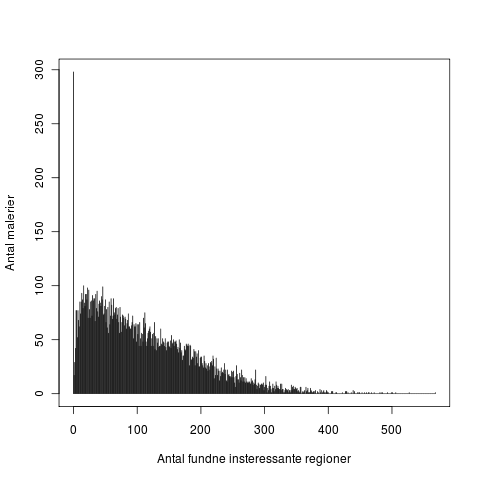
\includegraphics[width=0.49\textwidth]{afsnit/resultater/billeder/totalregions_var}
        \label{graf_total_regions_var}
    }
    \subfloat[]{
        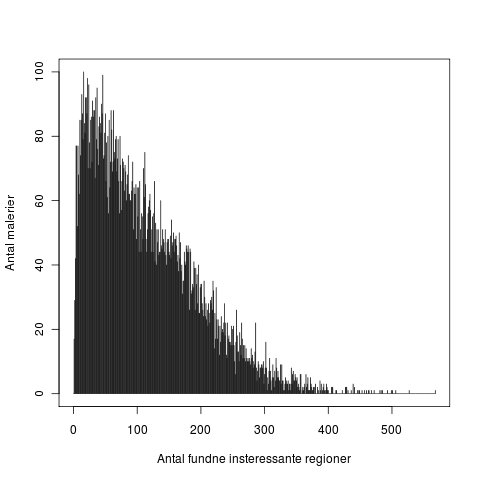
\includegraphics[width=0.49\textwidth]{afsnit/resultater/billeder/totalregions}
        \label{graf_total_regions_zoom}
    }
    \caption[]{Fordelingen af fundne regioner på malerier.
    \textbf{\ref{graf_total_regions_var}:} Plot som viser hvor mange
    malerier, hvori der er fundet et vist antal interessante regioner
    over alle snit i billedet.  \textbf{\ref{graf_total_regions_zoom}:}
    Samme plot som i figur \ref{graf_total_regions_var}, men hvor antal
    billeder uden regioner ikke er vist.}
    \label{total_regions_plots}
\end{figure}

\begin{figure}[!h]
    \centering
    \subfloat{
        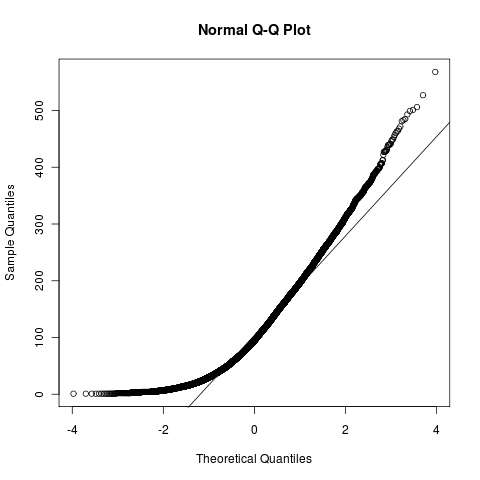
\includegraphics[width=0.49\textwidth]{afsnit/resultater/billeder/qq_totalregions}
        \label{qq_totalregions}
    }
    \subfloat[]{
        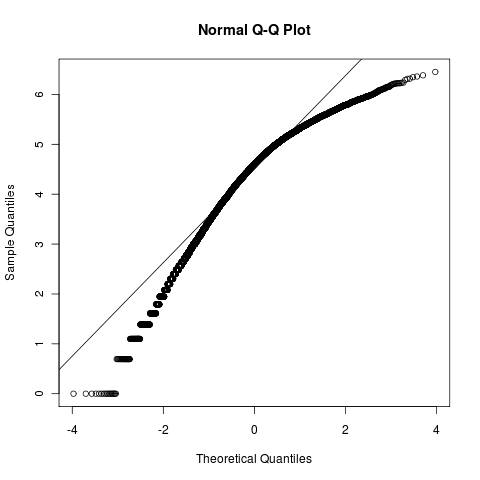
\includegraphics[width=0.49\textwidth]{afsnit/resultater/billeder/qq_log_totalregions}
        \label{qq_log_totalregions}
    }\\
    \subfloat[]{
        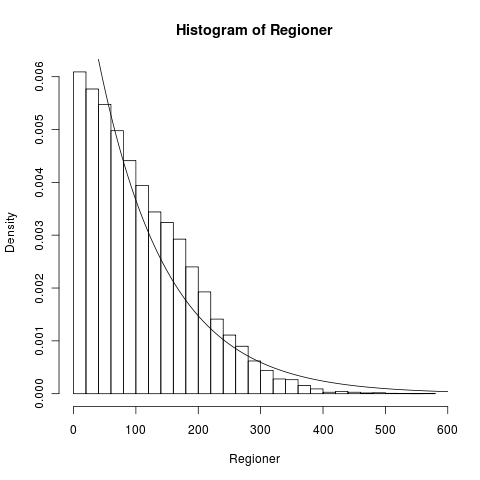
\includegraphics[width=0.62\textwidth]{afsnit/resultater/billeder/hist_totalregions}
        \label{hist_total_regions}
    }
    \caption[]{QQ-plots som ikke viser tegn på en normalfordeling af
    fundne regioner. \textbf{\ref{qq_totalregions}:} QQ-plot af antal
    billeder med én eller flere regioner.
    \textbf{\ref{qq_log_totalregions}:} Samme plot som i figur
    \ref{qq_totalregions}, men data er logaritmisk transformeret.
    \textbf{\ref{hist_total_regions}:} Histogram over antal fundne
    regioner med en eksponentialfordeling tegnet.}
    \label{qq_plots}
\end{figure}

}
% vim: set tw=72 spell spelllang=da:
